\newcommand{\shift}{\eta}
\newcommand{\vv}[1]{\boldsymbol{#1}}
\newcommand{\erep}{\mathbf{E}_{\epsilon}}
\newcommand{\eshift}{\mathbf{E}_{\shift}}
\newcommand{\ndata}{N_{\rm data}}
\newcommand\Fontvi{\fontsize{8}{7.2}\selectfont}

\makeatletter
\newcommand{\leqnomode}{\tagsleft@true\let\veqno\@@leqno}
\newcommand{\reqnomode}{\tagsleft@false\let\veqno\@@eqno}
\makeatother

\title{NNPDF}
\author[Michael Wilson]{}
\institute{University of Edinburgh}
\date{PDF4LHC}

\subsection{Closure testing NNPDF4.0}
\begin{frame}
    \frametitle{Closure Test}
    \Fontvi
    \begin{columns}[t]
    \column{0.5\textwidth}
    Fit replicas to pseudodata in usual way
    \leqnomode
    \begin{equation}\label{eq:dataassum}
    \begin{split}
        \vv{y} &= \vv{f} + \vv{\shift} + \vv{\epsilon} \\
        &= \vv{z} + \vv{\epsilon},
    \end{split}
    \end{equation}
    where $\vv{\shift} \sim \mathcal{N}(0, C)$ and $\vv{\epsilon} \sim \mathcal{N}(0, C)$ are sampled independently.
    
    Use predictions from an input PDF as proxy for $\vv{f}$.

    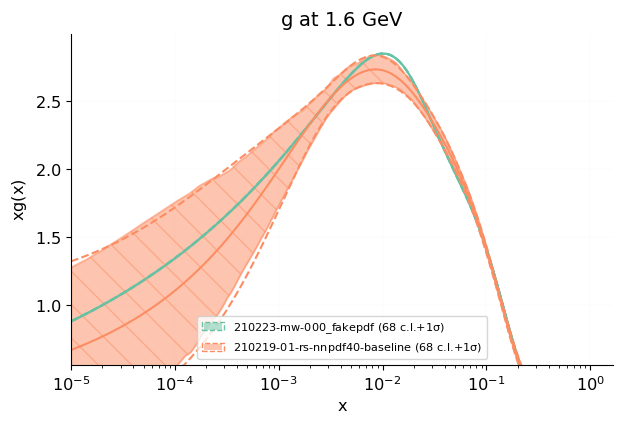
\includegraphics[scale=0.3]{closure_test/plot_pdfs_g.png}
    
    Sampling a random NNPDF replica as the input PDF for a closure test.
    \column{0.5\textwidth}
    \reqnomode
    Allows testing of methodology, if the input assumptions hold.

    \vspace{8pt}
    For example:
    \vspace{8pt}
    
    \textbf{Bias}: difference between central prediction and true observable

    \vspace{8pt}
    \textbf{Variance}: uncertainty of replica predictions

    \vspace{8pt}
    
    Bias is a stochastic variable. If PDF uncertainty is faithful then
    \begin{equation}
        \eshift[{\rm bias}] = {\rm variance}
    \end{equation}

    \vspace{8pt}
    
    High demand on resources - made feasible with \texttt{n3fit}
    \end{columns}
\end{frame}
%
\begin{frame}\frametitle{Preliminary results}
    \Fontvi
    Compare first moments:

    \begin{center}
    \begin{tabular}{lr}
        \toprule
        {} &  $\sqrt{\eshift[{\rm bias}] / \eshift[{\rm variance}]}$\\
        \midrule
        Total      & 1.11 $\pm$ 0.5 \\
        \bottomrule
        \end{tabular}
    \end{center}

    \vspace{8pt}
    Alternatively look at the respective distributions

    \vspace{8pt}
    \begin{center}
        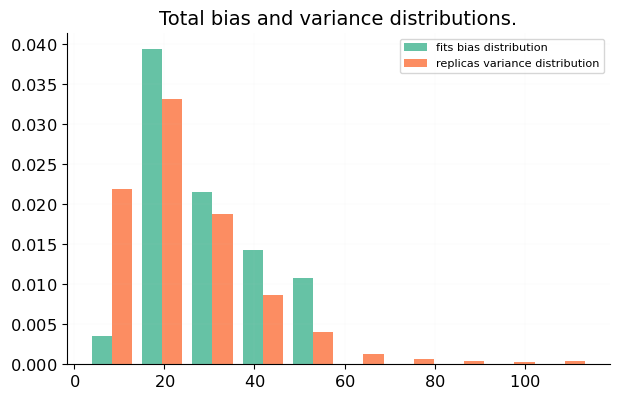
\includegraphics[scale=0.3]{closure_test/plot_bias_variance_distributions_3.png}
    \end{center}

    \vspace{8pt}
    Bias distribution sampled with 25 fits, 40 replicas each.

\end{frame}